% This is "sig-alternate.tex" V2.1 April 2013
% This file should be compiled with V2.5 of "sig-alternate.cls" May 2012
%
% This example file demonstrates the use of the 'sig-alternate.cls'
% V2.5 LaTeX2e document class file. It is for those submitting
% articles to ACM Conference Proceedings WHO DO NOT WISH TO
% STRICTLY ADHERE TO THE SIGS (PUBS-BOARD-ENDORSED) STYLE.
% The 'sig-alternate.cls' file will produce a similar-looking,
% albeit, 'tighter' paper resulting in, invariably, fewer pages.
%
% ----------------------------------------------------------------------------------------------------------------
% This .tex file (and associated .cls V2.5) produces:
%       1) The Permission Statement
%       2) The Conference (location) Info information
%       3) The Copyright Line with ACM data
%       4) NO page numbers
%
% as against the acm_proc_article-sp.cls file which
% DOES NOT produce 1) thru' 3) above.
%
% Using 'sig-alternate.cls' you have control, however, from within
% the source .tex file, over both the CopyrightYear
% (defaulted to 200X) and the ACM Copyright Data
% (defaulted to X-XXXXX-XX-X/XX/XX).
% e.g.
% \CopyrightYear{2007} will cause 2007 to appear in the copyright line.
% \crdata{0-12345-67-8/90/12} will cause 0-12345-67-8/90/12 to appear in the copyright line.
%
% ---------------------------------------------------------------------------------------------------------------
% This .tex source is an example which *does* use
% the .bib file (from which the .bbl file % is produced).
% REMEMBER HOWEVER: After having produced the .bbl file,
% and prior to final submission, you *NEED* to 'insert'
% your .bbl file into your source .tex file so as to provide
% ONE 'self-contained' source file.
%
% ================= IF YOU HAVE QUESTIONS =======================
% Questions regarding the SIGS styles, SIGS policies and
% procedures, Conferences etc. should be sent to
% Adrienne Griscti (griscti@acm.org)
%
% Technical questions _only_ to
% Gerald Murray (murray@hq.acm.org)
% ===============================================================
%
% For tracking purposes - this is V2.0 - May 2012

\documentclass{sig-alternate-05-2015}


\begin{document}

% Copyright
\setcopyright{acmcopyright}
%\setcopyright{acmlicensed}
%\setcopyright{rightsretained}
%\setcopyright{usgov}
%\setcopyright{usgovmixed}
%\setcopyright{cagov}
%\setcopyright{cagovmixed}


% DOI
\doi{10.475/123_4}

% ISBN
\isbn{123-4567-24-567/08/06}

%Conference
\conferenceinfo{PLDI '13}{June 16--19, 2013, Seattle, WA, USA}

\acmPrice{\$15.00}

%
% --- Author Metadata here ---
\conferenceinfo{WOODSTOCK}{'97 El Paso, Texas USA}
%\CopyrightYear{2007} % Allows default copyright year (20XX) to be over-ridden - IF NEED BE.
%\crdata{0-12345-67-8/90/01}  % Allows default copyright data (0-89791-88-6/97/05) to be over-ridden - IF NEED BE.
% --- End of Author Metadata ---

\title{A Failure Detection approach of Data Center Networks\titlenote{(Produces the permission block, and
copyright information). For use with
SIG-ALTERNATE.CLS. Supported by ACM.}}
%
% You need the command \numberofauthors to handle the 'placement
% and alignment' of the authors beneath the title.
%
% For aesthetic reasons, we recommend 'three authors at a time'
% i.e. three 'name/affiliation blocks' be placed beneath the title.
%
% NOTE: You are NOT restricted in how many 'rows' of
% "name/affiliations" may appear. We just ask that you restrict
% the number of 'columns' to three.
%
% Because of the available 'opening page real-estate'
% we ask you to refrain from putting more than six authors
% (two rows with three columns) beneath the article title.
% More than six makes the first-page appear very cluttered indeed.
%
% Use the \alignauthor commands to handle the names
% and affiliations for an 'aesthetic maximum' of six authors.
% Add names, affiliations, addresses for
% the seventh etc. author(s) as the argument for the
% \additionalauthors command.
% These 'additional authors' will be output/set for you
% without further effort on your part as the last section in
% the body of your article BEFORE References or any Appendices.

\numberofauthors{8} %  in this sample file, there are a *total*
% of EIGHT authors. SIX appear on the 'first-page' (for formatting
% reasons) and the remaining two appear in the \additionalauthors section.
%
\author{
% You can go ahead and credit any number of authors here,
% e.g. one 'row of three' or two rows (consisting of one row of three
% and a second row of one, two or three).
%
% The command \alignauthor (no curly braces needed) should
% precede each author name, affiliation/snail-mail address and
% e-mail address. Additionally, tag each line of
% affiliation/address with \affaddr, and tag the
% e-mail address with \email.
%
% 1st. author
\alignauthor
Kai Shen\titlenote{Dr.~Trovato insisted his name be first.}\\
       \affaddr{School of Software}\\
       \affaddr{Shanghai Jiao Tong University}\\
       \affaddr{Wallamaloo, New Zealand}\\
       \email{knshen@sjtu.edu.cn}
% 2nd. author
\alignauthor Charles Palmer\\
       \affaddr{Palmer Research Laboratories}\\
       \affaddr{8600 Datapoint Drive}\\
       \affaddr{San Antonio, Texas 78229}\\
       \email{cpalmer@prl.com}
}
% There's nothing stopping you putting the seventh, eighth, etc.
% author on the opening page (as the 'third row') but we ask,
% for aesthetic reasons that you place these 'additional authors'
% in the \additional authors block, viz.
% Just remember to make sure that the TOTAL number of authors
% is the number that will appear on the first page PLUS the
% number that will appear in the \additionalauthors section.

\maketitle
\begin{abstract}
This paper provides a sample of a \LaTeX\ document which conforms,
somewhat loosely, to the formatting guidelines for
ACM SIG Proceedings. It is an {\em alternate} style which produces
a {\em tighter-looking} paper and was designed in response to
concerns expressed, by authors, over page-budgets.
It complements the document \textit{Author's (Alternate) Guide to
Preparing ACM SIG Proceedings Using \LaTeX$2_\epsilon$\ and Bib\TeX}.
This source file has been written with the intention of being
compiled under \LaTeX$2_\epsilon$\ and BibTeX.

The developers have tried to include every imaginable sort
of ``bells and whistles", such as a subtitle, footnotes on
title, subtitle and authors, as well as in the text, and
every optional component (e.g. Acknowledgments, Additional
Authors, Appendices), not to mention examples of
equations, theorems, tables and figures.

To make best use of this sample document, run it through \LaTeX\
and BibTeX, and compare this source code with the printed
output produced by the dvi file. A compiled PDF version
is available on the web page to help you with the
`look and feel'.
\end{abstract}


%
% The code below should be generated by the tool at
% http://dl.acm.org/ccs.cfm
% Please copy and paste the code instead of the example below.
%
\begin{CCSXML}
<ccs2012>
 <concept>
  <concept_id>10010520.10010553.10010562</concept_id>
  <concept_desc>Computer systems organization~Embedded systems</concept_desc>
  <concept_significance>500</concept_significance>
 </concept>
 <concept>
  <concept_id>10010520.10010575.10010755</concept_id>
  <concept_desc>Computer systems organization~Redundancy</concept_desc>
  <concept_significance>300</concept_significance>
 </concept>
 <concept>
  <concept_id>10010520.10010553.10010554</concept_id>
  <concept_desc>Computer systems organization~Robotics</concept_desc>
  <concept_significance>100</concept_significance>
 </concept>
 <concept>
  <concept_id>10003033.10003083.10003095</concept_id>
  <concept_desc>Networks~Network reliability</concept_desc>
  <concept_significance>100</concept_significance>
 </concept>
</ccs2012>
\end{CCSXML}

\ccsdesc[500]{Computer systems organization~Embedded systems}
\ccsdesc[300]{Computer systems organization~Redundancy}
\ccsdesc{Computer systems organization~Robotics}
\ccsdesc[100]{Networks~Network reliability}


%
% End generated code
%

%
%  Use this command to print the description
%
\printccsdesc

% We no longer use \terms command
%\terms{Theory}

\keywords{ACM proceedings; \LaTeX; text tagging}

\section{Introduction}
Data center.
The rest of this paper is organized as follows. Section 2 discusses related work,

\section{Related Work}
In this section, we will present various relevant works including failure detectors, failure detection architecture in distributed systems and failure detection in data center networks.

\subsection{Failure Detectors}
A failure detector (FD) is widely recognized as an oracle to intelligently suspect failed processes \cite{chandra1996unreliable}. The monitored process periodically send heartbeat messages to its detector to prove its liveness.

Chen et al. proposed a FD that provides QoS \cite{chen2002quality}. It estimates the expected arrival time (EAs) of the next heartbeat message according to a slide window storing n most recent arrived messages. EAs determine the deadline that the detector will wait for the next heartbeat before suspecting the monitored process. \textit{Chen FD} can adjust current network condition and set the timeout threshold adaptively by referring to recent heartbeats. Bertier et al. proposed a similar FD \cite{bertier2002implementation}, whereas it uses a dynamic way to compute error margin of \textit{Chen FD}. Other FDs like \textit{$\phi$ Accrual FD} \cite{hayashibara2004varphi} and \textit{Satzger FD} \cite{satzger2007new} can output a continuous accrual failure value other than a binary value at any time which stands for the failure probability of the process.

\subsection{Failure Detection Architecture}
A failure detection architecture aims to provide the service of monitoring nodes in large scale distributed systems in a scalable way.
Roughly speaking, there are two kinds of architectures. The first one is hierarchical architecture \cite{felber1999failure}, all the nodes are partitioned into different groups, each group has a leader node. Within a group, the leader node is responsible for monitoring all the nodes. Leader nodes periodically send node status information of his group to other leader nodes. Hierarchical architecture can reduce the number of heartbeat messages effectively, but it exists \textit{Single Point of Failure} problem, when the leader node crashes, it needs to select a new leader.

Another alternative solution is Gossip-Style architecture \cite{van1998gossip}. Each node maintains a list containing the \textit{heartbeat counter} for each node in the system. Every T$_{gossip}$ seconds, each node firstly update \textit{heartbeat counter} of itself and then randomly select another node to send its list to. Upon receiving a message, the node will merge two lists and update each node's \textit{heartbeat counter} with the bigger one. If the \textit{heartbeat counter} does not update after T$_{fail}$ seconds, the node will be marked as crashed. If the \textit{heartbeat counter} does not update after T$_{cleanup}$ (T$_{cleanup}$
$\ge$T$_{fail}$) seconds, it will be removed from the list. This approach has very low bandwidth occupation because it only produces $n$ messages each epoch where $n$ is the size of the system. However, with the increasing of crashing nodes, it needs more time to detect these failures.

\subsection{Failure Detection in Networks}
Different from the work mentioned above, failure detection in networks should consider network topology and localize failure positions at IP layer. Gill et al. present the first large-scale survey on failures in data center networks \cite{gill2011understanding}.

Also, there exists a large body of work on applying statistical approaches to failure localization in networks. Sherlock \cite{bahl2007towards} localizes failures to limited network components by capturing dependencies between components. Shrink \cite{kandula2005shrink} leverages Bayesian Network model to diagnose root cause of IP network failures. Herodotou et al. \cite{herodotou2014scalable} actively inject ping traffic into network and analyze the ping results overlaid on top of the network topology. It will generate a ranked list containing the suspected failed device and links along with their failure score that can best explain the observed ping data.


\section{Data Center Network Architecture}
In this section, we will take a brief look at common data center network architecture.

A data center is a facility used to house computer systems and associated components, it usually contains hundreds of thousands devices and links. Modern data centers use hierarchical architecture. Figure 1 depicts a conventional data center network architecture \cite{gill2011understanding, greenberg2009vl2, herodotou2014scalable}. At the bottom layer are racks of servers, typically there are 20 to 40 servers in each rack, and each server in the same rack connects to a Top of Rack (ToR) Switch via a 1 Gbps link. Each ToR then connects to a primary and a backup Aggregation Switch (AS) for redundancy. ASs are connected to Access Routers (ARs) forming a complete bipartite graph. Finally, ARs are connected to Core Routers (CRs).

To limit overheads and to isolate different services, servers are partitioned into virtual LANs (VLANs). All links in the data center use Ethernet as link layer protocol and physical connections are a mix of copper and fiber cables. In addition to the devices in Figure 1, there may exist other devices like load balancers (LBs) and firewalls.

Modern data center usually employs \textit{Equal Cost MultiPath} (ECMP) routing within the data center for fault tolerance, which means that there are multiple paths from source to destination. Thus in this work, we will apply ECMP routing to the simulated network by enabling ECMP routing configurations in NS-3.

% figure
\begin{figure}
\centering
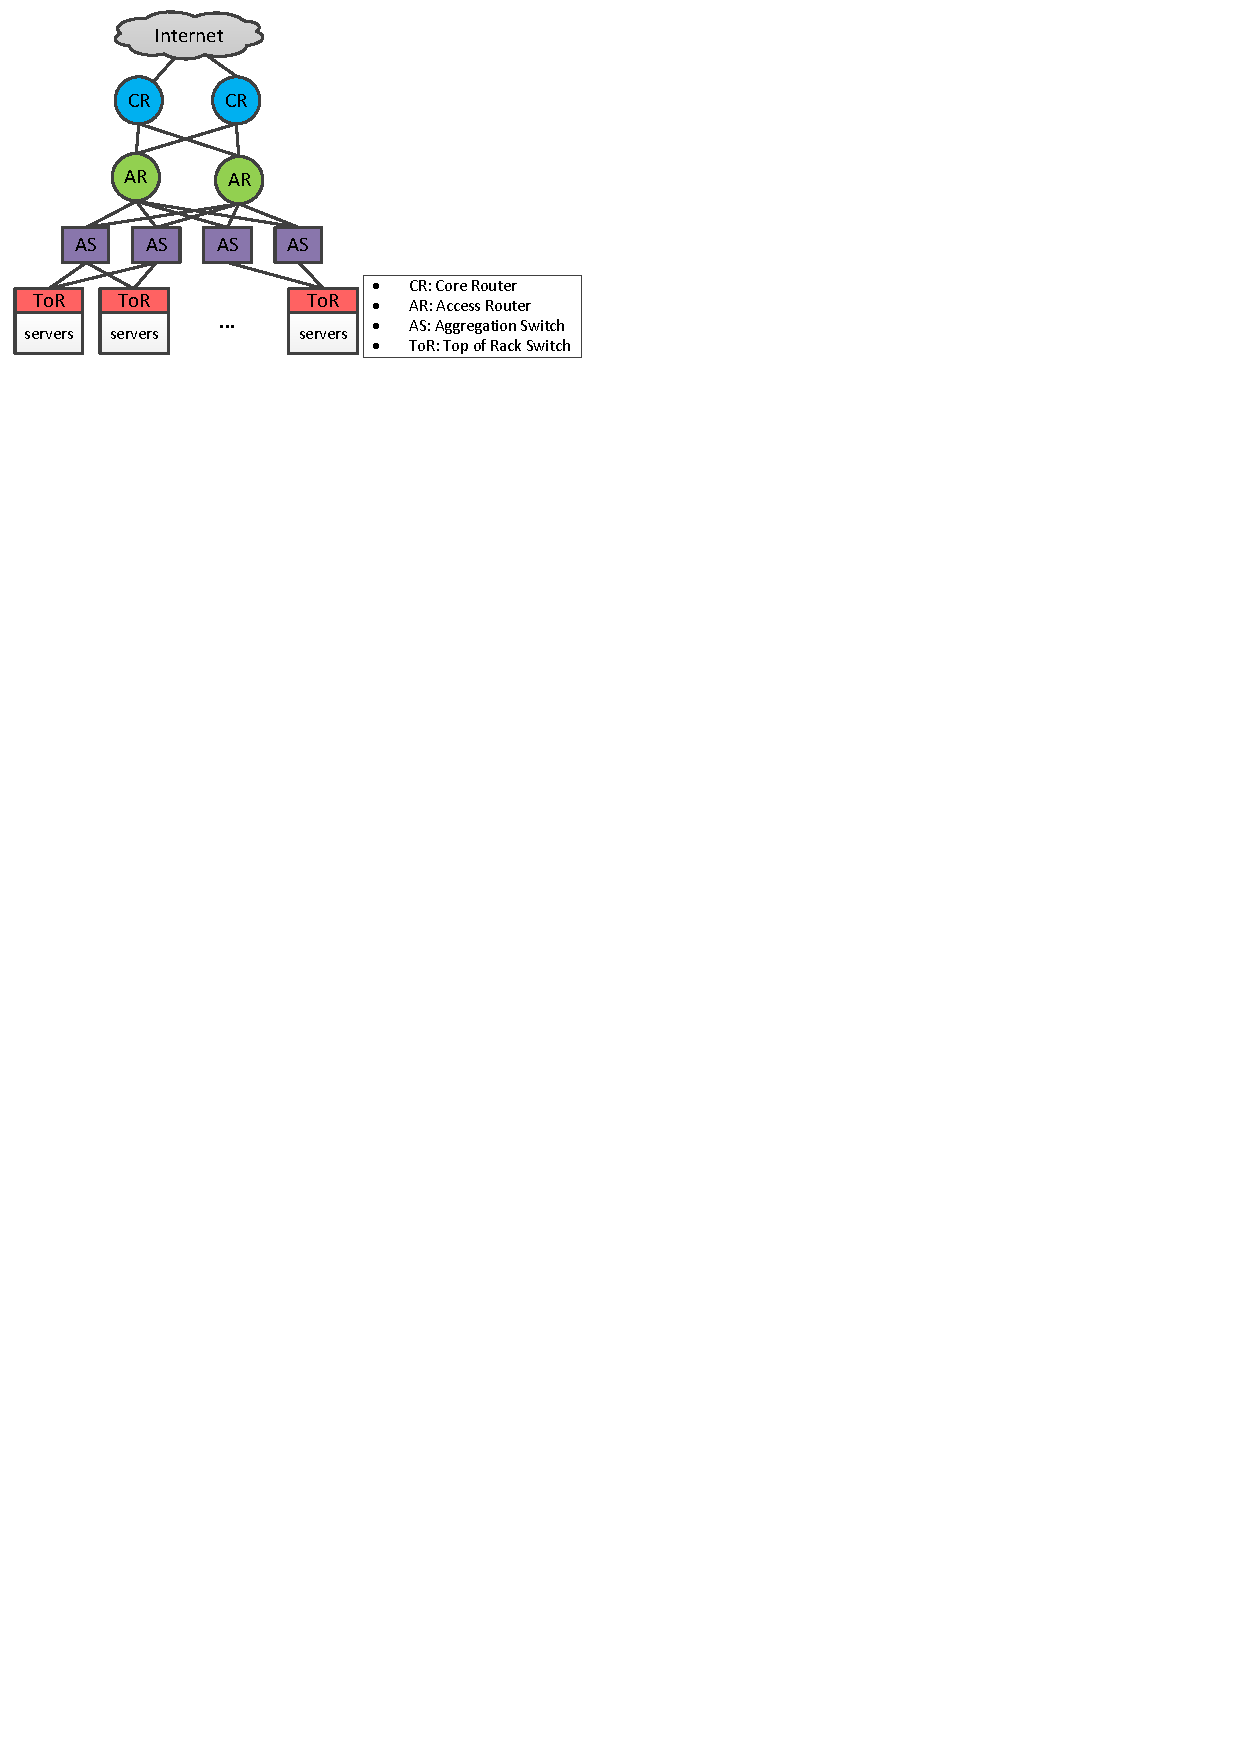
\includegraphics{topology}
\caption{Conventional Data Center Network Topology}
\end{figure}


\section{Approach Overview}
In this section, we will introduce the whole design of our failure detection approach.

Different network device should have different quality of service (QoS). Gill et.al \cite{gill2011understanding} have shown the diversity of different devices' failure characteristics. Unfortunately, none of the work in Section 2 treats these devices differently. We firstly divide network devices into two categories.

\begin{itemize}
\item \textbf{Imperetative Device.} This category includes servers, ToRs and links between ToRs and servers. Typically servers run various user applications and store user data. The crash of servers may cause user-perceived faults. The crash of a ToR will make servers under it unreachable. Also Gill et.al declare that the downtime of ToRs may be very long. Thus the failure detection for these devices must be fast enough besides the accuracy requirement.

\item \textbf{Non-imperetative Device.} It includes other routers and switches. A single failure of a link or a router does not affect the functionality of a data center because of path redundancy. So administrators care more about how effective the detect service is (The ability to identify actually happening failures).
    
\end{itemize}

% figure
\begin{figure}
\centering
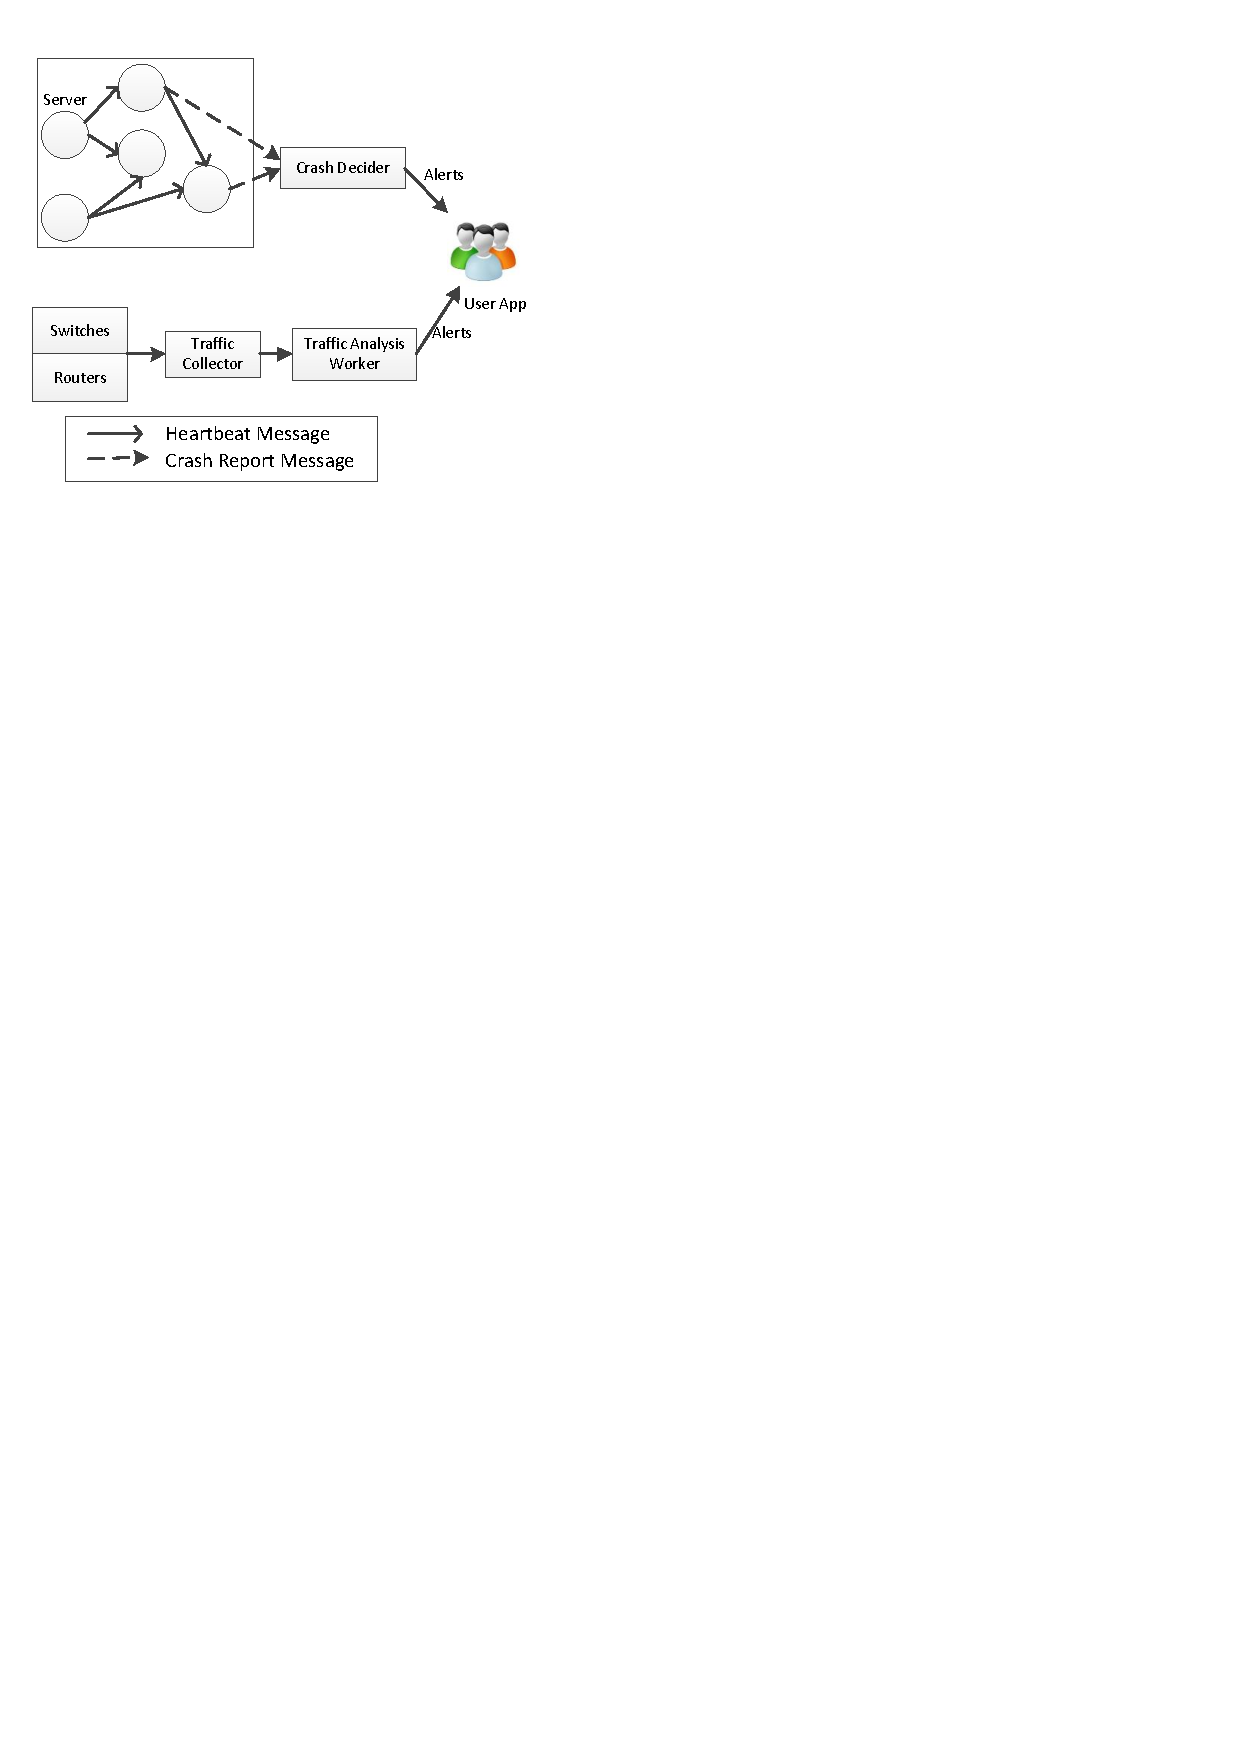
\includegraphics{system}
\caption{Failure Detection System Architecture}
\end{figure}

Figure 2 illustrates the entire architecture of our failure detection system. It mainly contains two modules. The servers failure detection system is autonomous and combines centralized structure with decentralized structure. A server can both play the role of a detector and a monitored object. Each server is monitored by multiple FD processes installed on different servers for redundancy. A server can also monitor a group of servers. Once the FD outputs the crash of a server, it will send a crash report message to \textbf{Crash Decider}. \textbf{Crash Decider} will determine the final status of this server.

For the detection of non-imperetative devices, \textbf{Traffic Collector} periodically collects traffic data of routers and switches and send telemetry data to \textbf{Traffic Analysis Worker}. \textbf{Traffic Analysis Worker} finally generate failure alerts by performing analysis on these data.

 

\section{Failure Detection Approach}
In this section, we will discuss the detailed design of different modules of the failure detection system respectively.

\subsection{Failure Detection for servers}
Failure Detection for servers is responsible for reporting the crash of servers effectively and efficiently. Our detection model is based on the assumption that once the server crashes, it never recovers by itself. The QoS of failure detection for servers are as follows:

\begin{itemize}
\item \textbf{Efficiency.} It measures how fast the system can report the crash of the server after it crashes. The system is more efficient if it takes less time to detect a failure.
\item \textbf{Completeness.} It measures whether the system can detect all the crashed servers. The system is more complete if it rules out fewer true crashed ones.
\item \textbf{Soundness.} In some scenarios, the behavior of the network may vary. For example, message loss and message delay may happen sometimes. The detection system should be sound enough to distinguish between such condition and a real crash.

\end{itemize}

\subsubsection{k-detector}
To meet the requirements mentioned above, this paper proposes a detector model named $k$-detector model which means each server is monitored by $k$ FDs on different servers whereas $k$ is a parameter tuned by users. \textbf{Crash Decider} only

\paragraph{Rationale}


\subsubsection{Monitoring Rule Inference}




\subsection{Failure Detection for ToRs}





\subsection{Failure Detection for Links}




\section{Evaluation}
In this section, we will present how we evaluate the efficiency and effectiveness of our approach as well as the experiments results.

\subsection{Experiments Setup}

\section{Conclusions}
This paper proposes a failure detector model for data center networks.
%\end{document}  % This is where a 'short' article might terminate


\section{Acknowledgments}
This work is partially supported by the National High-Technology Research and Development Program of China (Grant No.2014AA01A301).

%
% The following two commands are all you need in the
% initial runs of your .tex file to
% produce the bibliography for the citations in your paper.
\bibliographystyle{abbrv}
\bibliography{paper}  % sigproc.bib is the name of the Bibliography in this case
% You must have a proper ".bib" file
%  and remember to run:
% latex bibtex latex latex
% to resolve all references
%
% ACM needs 'a single self-contained file'!
%
%APPENDICES are optional
%\balancecolumns

\end{document}








